\section{Object-Oriented Programming (OOP)}

\subsection{Terms and Programming Concepts}

\begin{itemize}
    \item \textbf{Class:} A class is a blueprint for creating objects. It defines the attributes (variables) and methods (functions) that all instances of the class will have.
    
    \item \textbf{Instance:} An instance is a specific realization of a class. It is an individual object created from a class, with its own set of attributes and methods.
    
    \item \textbf{Attribute:} An attribute is a piece of data associated with a particular object. It can be thought of as a variable that belongs to an object.
    
    \item \textbf{Method:} A method is a function defined within a class. It operates on the data within the class and can modify the state of the object or perform some action.
    
    \item \textbf{Object:} In Python, everything is an object. An object is a collection of data (variables) and methods (functions) that act on the data.
    
    \item \textbf{Type:} The type of an object determines what class it belongs to. It defines the attributes and methods that the object will have.
\end{itemize}

\begin{codebox}
\begin{minted}{python}
# Define a Dog class
class Dog:
    # Constructor method to initialize object attributes
    def __init__(self, name, breed, age):
        self.name = name  
        self.breed = breed
        self.age = age

    # Method to get description of the dog
    def get_description(self):
        return f"{self.name} is a {self.age}-year-old {self.breed}."


# Create an instance of the Dog class
my_dog = Dog('Buddy', 'Golden Retriever', 3)

# Accessing age attribute directly
print(my_dog.age)  # Output: 3

# Call the get_description method to print dog's description
print(my_dog.get_description())

# Print the type of the object and the name of the class
print(type(my_dog))           # Output: <class '__main__.Dog'>
print(type(my_dog).__name__)  # Output: Dog
\end{minted}
\end{codebox}

\subsubsection{The \texttt{\_\_init\_\_()} method}

The \texttt{\_\_init\_\_} method is a special method used for initializing objects of a class. It is also known as a constructor method. The \texttt{\_\_init\_\_} method is called automatically whenever a new instance of the class is created.

\newpage
\subsubsection{Instance and Class Variables}

\begin{itemize}
\item \textbf{Instance Variables}\\
Variables that are unique to each instance of a class. They are defined within the constructor method (\texttt{\_\_init\_\_}) using the self keyword. Each instance of the class has its own copy of instance variables. Instance variables hold data that is specific to each object or instance of the class.

\item  \textbf{Class Variables}\\
Variables that are shared among all instances of a class. They are defined outside of any method, typically at the beginning of the class definition. Class variables are accessed using the class name itself, rather than through instances of the class. They are used to store data that is common to all instances of the class.
\end{itemize}

\begin{codebox}
\begin{minted}{python}
class Car:
    # Class variables
    wheels = 4
    total_cars = 0  # Counter for total number of cars

    def __init__(self, make, model):
        # Instance variables
        self.make = make
        self.model = model
        # Increment the total number of cars when a new instance is created
        Car.total_cars += 1


# Creating instances
car1 = Car('Toyota', 'Camry')
car2 = Car('Honda', 'Accord')
car3 = Car('Ford', 'Focus')

# Accessing class variable total_cars
print("Total number of cars:", Car.total_cars)  # Output: 3

# Accessing class variable using instance name (not recommended)
print(car1.total_cars) # Output: 3
\end{minted}
\end{codebox}

Although accessing class variables using an instance name works in Python, it's clearer and more conventional to access them using the class name directly. This helps to distinguish between instance variables and class variables clearly.

\newpage
\subsubsection{The \texttt{\_\_dict\_\_} Attribute}
The \texttt{\_\_dict\_\_} is a special attribute that is present in every object and holds the object's attributes. It is a dictionary that maps attribute names (as keys) to their corresponding values. You can use \texttt{\_\_dict\_\_} to access, manipulate, or inspect the attributes of an object dynamically.

\begin{codebox}
\begin{minted}{python}
class MyClass:
    class_variable = 0

    def __init__(self, x, y):
        self.x = x  
        self.y = y  


obj1 = MyClass(10, 20)

# Printing instance variables of obj1
print(obj1.__dict__)  # Output: {'x': 10, 'y': 20}

# Printing class variables and methods of MyClass
print(MyClass.__dict__)  # {'__module__': '__main__', 'class_variable': 0, ...
\end{minted}
\end{codebox}

\subsubsection{The \texttt{vars()} Function}

The \texttt{vars()} function is closely related to the \texttt{\_\_dict\_\_} attribute. It returns the \texttt{\_\_dict\_\_} attribute of an object if it exists, allowing you to access the object's attributes in the form of a dictionary. This function provides a convenient way to inspect the attributes of an object dynamically, similar to directly accessing the \texttt{\_\_dict\_\_} attribute.

\begin{codebox}
\begin{minted}{python}
class MyClass:
    class_variable = 0

    def __init__(self, x, y):
        self.x = x  
        self.y = y  


obj1 = MyClass(10, 20)

# Printing instance variables of obj1
print(vars(obj1))

# Printing class variables and methods of MyClass
print(vars(MyClass))
\end{minted}
\end{codebox}

\begin{minted}[
    bgcolor=white,
    frame=leftline,
    framesep=2mm,
    rulecolor=black,
    linenos=false, 
]{text}
{'x': 10, 'y': 20}
{
    '__module__': '__main__', 
    'class_variable': 0, 
    '__init__': <function MyClass.__init__ at 0x00000239ACED7600>, 
    '__dict__': <attribute '__dict__' of 'MyClass' objects>, ...
}
\end{minted}

%%%%%%%%%%%%%%%%%%%%%%%%%%%%%%%%%%%%%%%%%%%%%%%%%%%%%%%%%%%%%%%%%%%%%%%%%%
\newpage
\subsection{Core Syntax Operations}

\subsubsection{Magic Methods}
Magic methods, also known as dunder methods (short for "double underscore"), are special methods that have double underscore prefixes and suffixes, like \texttt{\_\_add\_\_}. These methods enable customization of how objects behave in certain contexts, such as arithmetic operations, comparison operations, and object creation.\\

\textbf{Comparison methods}\\[0.1cm]
\begin{tabular}{|p{3cm}|p{4cm}|p{8cm}|}
\hline
\textbf{Operator} & \textbf{Magic method} & \textbf{Implementation meaning or purpose} \\
\hline
\texttt{==} & \texttt{\_\_eq\_\_(self, other)} & Equality operator \\
\texttt{!=} & \texttt{\_\_ne\_\_(self, other)} & Inequality operator \\
\texttt{<} & \texttt{\_\_lt\_\_(self, other)} & Less-than operator \\
\texttt{>} & \texttt{\_\_gt\_\_(self, other)} & Greater-than operator \\
\texttt{<=} & \texttt{\_\_le\_\_(self, other)} & Less-than-or-equal-to operator \\
\texttt{>=} & \texttt{\_\_ge\_\_(self, other} & Greater-than-or-equal-to operator \\
\hline
\end{tabular}

\vspace{0.5cm}

\textbf{Unary operators and functions}\\[0.1cm]
\begin{tabular}{|p{3cm}|p{4cm}|p{8cm}|}
\hline
\textbf{Operator} & \textbf{Magic method} & \textbf{Implementation meaning or purpose} \\
\hline
\texttt{+} & \texttt{\_\_pos\_\_(self)} & Unary positive, like \texttt{a = +b} \\
\texttt{-} & \texttt{\_\_neg\_\_(self)} & Unary negative, like $a = -b$ \\
\texttt{abs()} & \texttt{\_\_abs\_\_(self)} & Behavior for \texttt{abs()} function \\
\texttt{round(a, b)} & \texttt{\_\_round\_\_(self, b)} & Behavior for \texttt{round()} function \\
\hline
\end{tabular}

\vspace{0.5cm}

\textbf{Common, binary operators and functions}\\[0.1cm]
\begin{tabular}{|p{2cm}|p{5cm}|p{8cm}|}
\hline
\textbf{Operator} & \textbf{Magic method} & \textbf{Implementation meaning or purpose} \\
\hline
\texttt{+} & \texttt{\_\_add\_\_(self, other)} & Addition operator \\
\texttt{-} & \texttt{\_\_sub\_\_(self, other)} & Subtraction operator \\
\texttt{*} & \texttt{\_\_mul\_\_(self, other)} & Multiplication operator \\
\texttt{//} & \texttt{\_\_floordiv\_\_(self, other)} & Integer division operator \\
\texttt{/} & \texttt{\_\_truediv\_\_(self, other)} & Division operator \\
\texttt{\%} & \texttt{\_\_mod\_\_(self, other)} & Modulo operator \\
\texttt{**} & \texttt{\_\_pow\_\_(self, other)} & Exponential (power) operator \\
\hline
\end{tabular}

\vspace{0.5cm}

\textbf{Augmented operators and functions}\\[0.1cm]
\begin{tabular}{|p{2cm}|p{5cm}|p{8cm}|}
\hline
\textbf{Operator} & \textbf{Magic method} & \textbf{Implementation meaning or purpose} \\
\hline
\texttt{+=} & \texttt{\_\_iadd\_\_(self, other)} & Addition and assignment operator \\
\texttt{-=} & \texttt{\_\_isub\_\_(self, other)} & Subtraction and assignment operator \\
\texttt{*=} & \texttt{\_\_imul\_\_(self, other)} & Multiplication and assignment operator \\
\texttt{//=} & \texttt{\_\_ifloordiv\_\_(self, other)} & Integer division and assignment operator \\
\texttt{/=} & \texttt{\_\_idiv\_\_(self, other)} & Division and assignment operator \\
\texttt{\%=} & \texttt{\_\_imod\_\_(self, other)} & Modulo and assignment operator \\
\texttt{**=} & \texttt{\_\_ipow\_\_(self, other)} & Exponential (power) and assignment operator \\
\hline
\end{tabular}
\vspace{0.5cm}

\newpage
\textbf{Type conversion methods}\\[0.1cm]
\begin{tabular}{|p{2cm}|p{4cm}|p{9cm}|}
\hline
\textbf{Function} & \textbf{Magic method} & \textbf{Implementation meaning or purpose} \\
\hline
\texttt{int()} & \texttt{\_\_int\_\_(self)} & Conversion to integer type \\
\texttt{float()} & \texttt{\_\_float\_\_(self)} & Conversion to float type \\
\texttt{oct()} & \texttt{\_\_oct\_\_(self)} & Conversion to string, containing an octal representation \\
\texttt{hex()} & \texttt{\_\_hex\_\_(self)} & Conversion to string, containing a hex representation \\
\hline
\end{tabular}

\vspace{0.5cm}

\textbf{Object introspection}\\[0.1cm]
\begin{tabular}{|p{2cm}|p{5.5cm}|p{7.5cm}|}
\hline
\textbf{Function} & \textbf{Magic method} & \textbf{Implementation meaning or purpose} \\
\hline
\texttt{str()} & \texttt{\_\_str\_\_(self)} & Handling str() function calls \\
repr() & \texttt{\_\_repr\_\_(self)} & Handling repr() function calls \\
\texttt{format()} & \texttt{\_\_format\_\_(self, formatstr)} & When string formatting is applied to an object \\
\texttt{hash()} & \texttt{\_\_hash\_\_(self)} & Handling hash() function calls \\
\texttt{dir()} & \texttt{\_\_dir\_\_(self)} & Handling dir() function calls \\
\texttt{bool()} & \texttt{\_\_nonzero\_\_(self)} & Handling bool() calls (\texttt{\_\_bool\_\_()} in Python 3)
 \\
\hline
\end{tabular}

\vspace{0.5cm}

\textbf{Object retrospection}\\[0.1cm]
\begin{tabular}{|p{4.5cm}|p{6cm}|p{4.5cm}|}
\hline
\textbf{Function} & \textbf{Magic method} & \textbf{Implementation} \\
\hline
\texttt{isinstance(obj, class)} & \texttt{\_\_instancecheck\_\_(self, obj)} & Handling isinstance() calls \\
\texttt{issubclass(subclass, class)} & \texttt{\_\_subclasscheck\_\_(self, subclass)} & Handling issubclass() calls \\
\hline
\end{tabular}

\vspace{0.5cm}

\textbf{Object attribute access}\\[0.1cm]
\begin{tabular}{|p{3.5cm}|p{6cm}|p{5.5cm}|}
\hline
\textbf{Expression} & \textbf{Magic method} & \textbf{Implementation} \\
\hline
\texttt{obj.attr} & \texttt{\_\_getattr\_\_(self, attr)} & Access to a non-existing attribute \\
\texttt{obj.attr} & \texttt{\_\_getattribute\_\_(self, attr)} & Access to an existing attribute \\
\texttt{obj.attr = val} & \texttt{\_\_setattr\_\_(self, attr, val)} & Setting an attribute value \\
\texttt{del object.attr} & \texttt{\_\_delattr\_\_(self, attr)} & Deleting an attribute \\
\hline
\end{tabular}

\vspace{0.5cm}

\textbf{Methods allowing access to containers}\\[0.1cm]
\begin{tabular}{|p{4.5cm}|p{6cm}|p{4.5cm}|}
\hline
\textbf{Expression} & \textbf{Magic method} & \textbf{Implementation} \\
\hline
\texttt{len(container)} & \texttt{\_\_len\_\_(self)} & Returns number of elements of the container \\
container[key] & \texttt{\_\_getitem\_\_(self, key)} & Fetching an element identified by the key\\
\texttt{container[key] = value} & \texttt{\_\_setitem\_\_(self, key, value)} & Setting a value to an element identified by the key\\
\texttt{del container[key]} & \texttt{\_\_delitem\_\_(self, key)} & Deleting an element identified by the key\\
\texttt{for el in container} & \texttt{\_\_iter\_\_(self)} & Returns an iterator for the container \\
\texttt{item in container} & \texttt{\_\_contains\_\_(self, item)} & Returns true if container has the item \\
\hline
\end{tabular}

\vspace{0.5cm}





By implementing these methods in a class, you can customize how instances of the class behave in various contexts, making your code more expressive and idiomatic.

\newpage
\subsubsection{Comparison Methods}

This code demonstrates the use of the \texttt{\_\_eq\_\_} method in classes, along with the behavior of the equality operator (\texttt{==}).

\begin{codebox}
\begin{minted}{python}
class Point():
    def __init__(self, x, y):
        self.x = x
        self.y = y
        
    def __eq__(self, other):
        return (self.x, self.y) == (other.x, other.y)

point1=Point(1,2)
point2=Point(1,2)

print(point1.__eq__(point2))  # Output: True
print(point1 == point2)  # Output: True
\end{minted}
\end{codebox}

\subsubsection{Accessing Containers}

The \texttt{\_\_getitem\_\_} method is a special method that allows objects to support indexing and slicing operations. It is called when you use square brackets (\texttt{[]}) to access elements from a container object, such as lists, dictionaries, or custom classes.

\begin{codebox}
\begin{minted}{python}
class MyContainer:
    def __init__(self, data):
        self.data = data

    def __getitem__(self, index):
        return self.data[index]

container = MyContainer([1, 2, 3, 4, 5])
print(container[2])  # Output: 3
\end{minted}
\end{codebox}

\subsubsection{Numeric Methods}
The \texttt{\_\_abs\_\_()} method is a special method that allows objects to define custom behavior for the built-in \texttt{abs()} function when applied to instances of the class.

\begin{codebox}
\begin{minted}{python}
class MyNumber:
    def __init__(self, value):
        self.value = value
    
    def __abs__(self):
        return abs(self.value)

x = MyNumber(-5)
print(abs(x))  # Output: 5
\end{minted}
\end{codebox}

\newpage
\subsubsection{Customizing Object Behavior}

The methods \texttt{\_\_call\_\_}, \texttt{\_\_repr\_\_}, and \texttt{\_\_str\_\_} are special methods that allow to customize the behavior of objects.

\begin{itemize}
    \item \textbf{The \_\_call\_\_ method:} allows the instance of \texttt{MyClass} to behave like a function. It is called when an instance of the class is used as if it were a function, for example, \texttt{obj()}.
    \item \textbf{The \_\_repr\_\_ method:} provides an unambiguous representation of the object, primarily meant for developers. It should ideally be valid Python code to recreate the object. It is used for debugging, logging, or creating new instances of the object.
    \item \textbf{The \_\_str\_\_ method:} provides a more user-friendly string representation of the object. It is called when the built-in function \texttt{str()} is used on the object, or when the object is passed to the \texttt{print()} function.
\end{itemize}

\begin{codebox}
\begin{minted}{python}
class MyClass:
    def __init__(self, x):
        self.x = x

    def __call__(self, y):
        # Allows instances of a class to be invoked like functions
        return self.x + y

    def __repr__(self):
        # Returns a string representation for developers
        return f'MyClass({self.x})'

    def __str__(self):
        # Returns a user-friendly string representation of the object
        return f'MyClass object with x = {self.x}'

# Creating an instance of MyClass
obj = MyClass(5)

# Using __call__ method
print(obj(3))

# Using __repr__ method
print(repr(obj))
print([obj]) # Calls __repr__ for each object in the list
logging.error(repr(obj)) # Using repr() for debugging/logging
#print(`obj`)  # Equivalent to repr(obj), in Python 2.x

# Using __str__ method, calls obj.__repr__() if __str__ is not defined
print(obj) 
print(str(obj))
print(f'{obj}')
print("%s" % obj)
print("{}".format(obj))
print(MyClass(2))
\end{minted}
\end{codebox}

\newpage
\subsubsection{Object Attribute Access}
The \_\_getattr\_\_, \_\_setattr\_\_, and \_\_delattr\_\_ methods are special methods that allow you to customize attribute access, assignment, and deletion behavior in objects.

\begin{itemize}
    \item \textbf{\texttt{\_\_getattr\_\_}}: This method is called when an attribute lookup fails. It allows you to define custom behavior for accessing attributes that don't exist in an object's namespace.
    
    \item \textbf{\texttt{\_\_setattr\_\_}}: This method is called when an attribute assignment is made. It allows you to customize behavior when setting attributes.
    
    \item \textbf{\texttt{\_\_delattr\_\_}}: This method is called when an attribute deletion is requested. It allows you to customize behavior when deleting attributes.
\end{itemize}

\begin{codebox}
\begin{minted}{python}
class DynamicAttributes:
    def __init__(self):
        self.data = {}

    def __getattr__(self, name):
        if name in self.data:
            return self.data[name]
        else:
            raise AttributeError(f"Object has no attribute '{name}'")

    def __setattr__(self, name, value):
        print(f"Setting attribute '{name}' to '{value}'")
        self.data[name] = value

    def __delattr__(self, name):
        if name in self.data:
            del self.data[name]
            print(f"Deleted attribute '{name}'")
        else:
            raise AttributeError(f"Object has no attribute '{name}'")


# Creating an instance of DynamicAttributes
obj = DynamicAttributes()

# Setting attribute
obj.x = 10  # Output: Setting attribute 'x' to '10'

# Accessing attribute
print(obj.x)  # Output: 10

# Deleting attribute
del obj.x  # Output: Deleted attribute 'x'

# Trying to access deleted attribute
print(obj.x)  # Raises AttributeError
\end{minted}
\end{codebox}

% TODO
%\subsubsection{Object intro- and retrospection}

%\subsubsection{Extending class implementations to support additional core syntax operations}

%%%%%%%%%%%%%%%%%%%%%%%%%%%%%%%%%%%%%%%%%%%%%%%%%%%%%%%%%%%%%%%%%%%%%%%%%%
\newpage
\subsection{Inheritance, Polymorphism, and Composition}

\subsubsection{Superclasses and Subclasses}
\begin{itemize}
    \item \textbf{Superclasses:}
    Provide a blueprint or template for the subclasses to follow.
    \item \textbf{Subclasses:}
    Inherit properties (attributes) and behaviors (methods) from their superclasses.
\end{itemize}

\begin{codebox}
\begin{minted}{python}
class Animal:
    def speak(self):
        print("This animal makes a sound.")

class Dog(Animal):
    def speak(self):
        print("Woof!")

class Cat(Animal):
    def speak(self):
        print("Meow!")


# Create instances of Dog and Cat
dog = Dog()
cat = Cat()
\end{minted}
\end{codebox}
The code defines three classes: \texttt{Animal}, \texttt{Dog}, and \texttt{Cat}. The \texttt{Animal} class has a method named \texttt{speak} that prints "This animal makes a sound." Both the \texttt{Dog} and \texttt{Cat} classes are subclasses of \texttt{Animal}, inheriting the \texttt{speak} method. The \texttt{Dog} class overrides the \texttt{speak} method with its own implementation to print "Woof!", and similarly, the \texttt{Cat} class overrides the \texttt{speak} method with its own implementation to print "Meow!".

\subsubsection{Reflection: \texttt{isinstance()} and \texttt{issubclass()}}

Reflection refers to the ability of a program to examine and modify its own structure, behavior, and metadata at runtime. This includes the capability to inspect classes, functions, modules, and objects to retrieve information about their attributes, methods, and other properties

\begin{itemize}
    \item \textbf{Introspection}: Examining the type and structure of objects at runtime.
    \item \textbf{Dynamic instantiation}: Creating instances of classes dynamically, based on runtime information.
    \item \textbf{Attribute and method manipulation}: Accessing and modifying attributes and methods of objects dynamically.
    \item \textbf{Dynamic module loading}: Loading modules dynamically during program execution.
    \item \textbf{Metaprogramming}: Writing code that generates or modifies other code.
\end{itemize}

\newpage
The \texttt{isinstance()} and \texttt{issubclass()} function are two built-in functions in Python used for type checking and inheritance checking respectively.

\begin{itemize}
\item \textbf{\texttt{isinstance()}:} This function is used to check if an object belongs to a particular class or any subclass of that class. It takes two arguments: the object and the class (or a tuple of classes). It returns True if the object is an instance of the specified class or any of its subclasses, otherwise, it returns False.
\begin{codebox}
\begin{minted}{python}
print(isinstance(dog, Animal))  # Output: True
print(isinstance(dog, Dog))     # Output: True
print(isinstance(cat, Dog))     # Output: False
\end{minted}
\end{codebox}

\item \textbf{\texttt{issubclass()}:} This function is used to check if a class is a subclass of another class. It takes two arguments: the subclass and the superclass. It returns True if the first class is indeed a subclass of the second class, otherwise, it returns False. Reflection enables dynamic manipulation of code and data structures, allowing for tasks such as:

\begin{codebox}
\begin{minted}{python}
print(issubclass(Dog, Animal))  # Output: True
print(issubclass(Cat, Animal))  # Output: True
print(issubclass(Cat, Cat))     # Output: True
\end{minted}
\end{codebox}

Cat is a subclass of Animal, and \texttt{issubclass(Cat, Cat)} correctly outputs \texttt{True} because a class is considered a subclass of itself. This behavior is expected in Python.
\end{itemize}

\subsubsection{Introspection}
Introspection refers to the ability of a program to examine the type, properties, and methods of objects at runtime. It allows you to dynamically inspect and manipulate objects, classes, functions, and modules within your code. Python's introspection capabilities are facilitated by various built-in functions and modules that provide information about objects. Some of the commonly used functions and modules for introspection include:

\begin{itemize}
    \item \textbf{type():} Returns the type of an object.
    \item \textbf{dir():} Returns a list of attributes and methods of an object.
    \item \textbf{getattr():} Retrieves the value of an attribute of an object dynamically, based on its name.
    \item \textbf{hasattr():} Checks whether an object has a specific attribute.
    \item \textbf{callable():} Checks whether an object is callable (i.e., whether it can be called as a function).
    \item \textbf{help():} Provides interactive help on objects, modules, functions, classes, and methods.
\end{itemize}

\begin{codebox}
\begin{minted}{python}
class Cat:
    def __init__(self, name, color):
        self.name = name
        self.color = color

my_cat = Cat("Whiskers", "gray")

# Example using getattr and hasattr
print(getattr(my_cat, "name"))  # Output: Whiskers
print(hasattr(my_cat, "name"))   # Output: True
print(hasattr(my_cat, "age"))    # Output: False
\end{minted}
\end{codebox}


\newpage
\subsubsection{Inheritance vs. Composition}
In object-oriented programming, inheritance and composition are two fundamental concepts used for structuring and organizing code.\\

\begin{itemize}
\item \textbf{Inheritance}: A new class (subclass or derived class) is created by inheriting properties and behaviors from an existing class (superclass or base class). It promotes code reusability by allowing subclasses to inherit attributes and methods from a superclass. Subclasses can then add their own attributes and methods or override the ones inherited from the superclass.

\begin{codebox}
\begin{minted}{python}
class Vehicle:
    def drive(self):
        return "Vehicle is being driven"

class Car(Vehicle):
    def drive(self):
        return "Car is being driven"
\end{minted}
\end{codebox}


\item \textbf{Composition}: A class contains objects of other classes as members. Instead of inheriting their behavior, the containing class delegates tasks to contained objects. It allows for building complex objects by combining simpler ones. Each object maintains its own behavior, and the containing object orchestrates their interactions.

\begin{codebox}
\begin{minted}{python}
class Engine:
    def start(self):
        return "Engine started"

class Car:
    def __init__(self):
        self.engine = Engine()
        
    def start(self):
        return self.engine.start()
\end{minted}
\end{codebox}
\end{itemize}

\subsubsection{Real-life problems using "is a" and "has a" relations}

\begin{itemize}
\item \textbf{Inheritance: "is-a" Relationship}\\
Subclasses are specialized versions of their superclass. Subclasses inherit common properties and behaviors from their superclass. For example, a Car is a type of Vehicle.\\

\item \textbf{Composition: "has-a" Relationship}\\
Classes contain instances of other classes as components. This allows them to utilize the functionalities of those components. For example, a Car has an Engine, Wheel, and Transmission.
\end{itemize}

\newpage
\subsubsection{Class Hierarchies}
Class hierarchies are structures that organize classes into a tree-like hierarchy, where classes can inherit attributes and methods from their parent classes. This enables code reuse, modularity, and the implementation of polymorphism.

\subsubsection{Single vs. Multiple Inheritance}
Inheritance allows a class to inherit attributes and methods from another class. There are two types of inheritance: single inheritance and multiple inheritance.\\

\begin{itemize}
\item \textbf{Single Inheritance:}
Class inherits from only one base class.\\

\begin{codebox}
\begin{minted}{python}
class Animal:
    def sleep(self):
        return "Animal sleeps"

class Dog(Animal):
    def bark(self):
        return "Dog barks"


dog = Dog()

# Dog inherits from Animal
# Dog class has access to the methods of Animal class
print(dog.sleep())  # Output: "Animal sleeps"
print(dog.bark())   # Output: "Dog barks"
\end{minted}
\end{codebox}

\item \textbf{Multiple Inheritance:}
Class inherits from multiple base classes.\\


\begin{codebox}
\begin{minted}{python}
class Animal:
    def sleep(self):
        return "Animal sleeps"

class Pet:
    def play(self):
        return "Pet plays"

class Dog(Animal, Pet):
    def bark(self):
        return "Dog barks"


dog = Dog()

# Dog inherits from both Animal and Pet
# Dog class has access to the methods of Animal and Pet classes
print(dog.sleep())  # Output: "Animal sleeps"
print(dog.play())   # Output: "Pet plays"
print(dog.bark())   # Output: "Dog barks"
\end{minted}
\end{codebox}
\end{itemize}

\newpage
\subsubsection{Polymorphism}
Polymorphism refers to the ability of different objects to respond to the same method or function call in different ways. It allows objects of different classes to be treated as objects of a common superclass, enabling code reuse and flexibility in design. There are two main types of polymorphism:

\begin{itemize}
    \item \textbf{Method Overriding:} This occurs when a subclass provides a specific implementation of a method that is already defined in its superclass. The method in the subclass overrides the method with the same name and signature in the superclass.
    
    \item \textbf{Operator Overloading:} This allows operators to have different implementations depending on the types of operands involved. Python provides special methods, often referred to as "magic methods" or "dunder methods", to enable operator overloading.
\end{itemize}

\subsubsection{Duck Typing}
Duck typing is a concept, where the type or class of an object is determined not by its inheritance hierarchy or explicit declaration, but by its behavior. In other words, an object's suitability is determined by whether it behaves like a duck, if it walks like a duck and quacks like a duck, then it must be a duck.
This means that if an object supports the necessary methods or attributes required by a particular operation, it can be used in that context regardless of its actual class or inheritance.

\begin{codebox}
\begin{minted}{Python}
class Duck:
    def quack(self):
        print("Quack!")

class Robot:
    def quack(self):
        print("I'm quacking like a duck!")

def make_it_quack(obj):
    obj.quack()

# Instances of Duck and Robot
duck = Duck()
robot = Robot()

# Duck typing allows any object with a quack() method
make_it_quack(duck)   # Output: "Quack!"
make_it_quack(robot)  # Output: "I'm quacking like a duck!"
\end{minted}
\end{codebox}

\begin{figure}[h!]
    \centering
    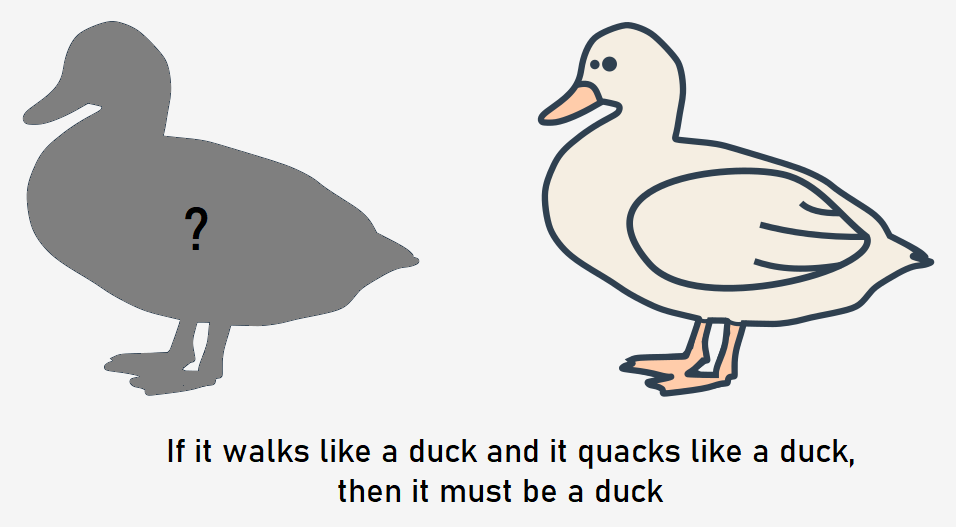
\includegraphics[width=0.4\textwidth]{images/twoDucks.png}
    \caption{Duck typing}
    \label{fig:example-1}
\end{figure}

%\begin{quote}
%\textit{``If it looks like a duck, swims like a duck, and quacks like a duck, \\ then it probably is a duck.''}
%\end{quote}


\newpage
\subsubsection{Diamond Problem: Method Resolution Order (MRO)}
The Diamond problem does not exist in Python because it gives preference to the class that is inherited first. The Method Resolution Order (MRO) defines the order in which Python looks for methods and attributes in a class hierarchy. When a method is called on an object, Python searches for it starting from the class of the object and then follows the MRO to find the method in the inheritance hierarchy.

\begin{codebox}
\begin{minted}{python}
class A:
    def hello(self):
        print('Hello from class A')
 
class B(A):
    def hello(self):
        print('Hello from class B')
 
class C(A):
    def hello(self):
        print('Hello from class C')
 
class D(B, C):
    pass

D().hello()  # Output: Hello from class B
\end{minted}
\end{codebox}

\texttt{D().hello()} calls the \texttt{hello()} method of class D. Since class D doesn't have its own \texttt{hello()} method, Python looks for it in the classes D inherits from, following the MRO. Therefore, the output of \texttt{D().hello()} is "Hello from class B".

\begin{codebox}
\begin{minted}{python}
# Output the MRO for class D
print(D.__mro__)
\end{minted}
\end{codebox}
\begin{minted}[
    bgcolor=white,
    frame=leftline,
    framesep=2mm,
    rulecolor=black,
    linenos=false,
]{text}
(__main__.D, __main__.B, __main__.C, __main__.A, object)
\end{minted}

Python will look for the \texttt{hello} method in class D first, then in class B, then in class C, then in class A, and finally in the base class \texttt{object}. Given the provided class hierarchy, the MRO for class D is as follows: 
$D \to B \to C \to A \to \texttt{object}$\\

\newpage
\subsubsection{The Inheritance Tangle}
The diamond inheritance problem is a common challenge encountered in object-oriented programming, particularly in languages like Python that support multiple inheritance. This issue arises when a class inherits from two or more classes, each of which in turn inherits from a common base class. As a result, the inheritance hierarchy forms a diamond shape, with multiple paths leading to the same base class.

\begin{codebox}
\begin{minted}{python}
class A:
    def info(self):
        print('Class A')

class B(A):
    def info(self):
        print('Class B')

class MyClass(A, B):
    pass

MyClass().info()
\end{minted}
\end{codebox}

\begin{minted}[
    bgcolor=white,
    frame=leftline,
    framesep=2mm,
    rulecolor=black,
    linenos=false, 
]{text}
---------------------------------------------------------------------------
TypeError                                 Traceback (most recent call last)
Cell In[24], line 9
      6     def info(self):
      7         print('Class B')
----> 9 class MyClass(A, B):
     10     pass
     12 MyClass().info()

TypeError: Cannot create a consistent method resolution
order (MRO) for bases A, B
\end{minted}

The error encountered stems from the diamond inheritance problem in Python. When a class like \texttt{MyClass(A, B)} is defined, inheriting from both \texttt{A} and \texttt{B}, Python faces difficulty in establishing a consistent method resolution order (MRO) due to conflicting inheritance paths. In this scenario, both \texttt{A} and \texttt{B} serve as base classes for \texttt{MyClass}, sharing a common ancestor (\texttt{object} by default in Python 3). However, Python's MRO algorithm struggles to determine a linear order for method search amidst these conflicting paths.\\

To resolve this error, it's necessary to redesign the class hierarchy to avoid the diamond inheritance problem. A common approach involves ensuring that each class inherits from its base classes via a single, unambiguous path.


\newpage
\subsubsection{The \texttt{super()} Function}
\texttt{super()} is a built-in function that allows you to call methods and access attributes from the parent class within a subclass. It provides a way to invoke methods defined in the superclass (parent class) of an object, enabling better code reuse and maintaining a clean inheritance structure.\\

The \texttt{super()} function is typically used inside methods of a subclass to call the corresponding method of the superclass. This is particularly useful when the subclass overrides a method defined in the superclass but still wants to execute the overridden method's behavior. By using \texttt{super()}, you can avoid explicitly naming the parent class and make your code more flexible to changes in the inheritance hierarchy.

\begin{codebox}
\begin{minted}{python}
class Parent:
  def __init__(self, msg):
    print("Calling Parent class constructor")
    self.message = msg

  def printmessage(self):
    print(self.message)

class Child(Parent):
  def __init__(self, msg):
    print("Calling Child class constructor")
    super().__init__(msg)


obj = Child("Hello, and welcome!")
obj.printmessage()
\end{minted}
\end{codebox}

\begin{minted}[
    bgcolor=white,
    frame=leftline,
    framesep=2mm,
    rulecolor=black,
    linenos=false,
]{text}
Calling Child class constructor
Calling Parent class constructor
Hello, and welcome!
\end{minted}

%%%%%%%%%%%%%%%%%%%%%%%%%%%%%%%%%%%%%%%%%%%%%%%%%%%%%%%%%%%%%%%%%%%%%%%%%%
% 1.8
\newpage
\subsubsection{Subclassing Built-in Classes}
%\subsubsection{Inheriting properties from built-in classes}
Inheriting properties from built-in classes allows for flexible customization of classes to suit specific needs without having to start from scratch. This is often done to customize behavior, add functionality, or override existing methods. However, it's essential to be cautious when subclassing built-ins, as it may lead to unexpected behavior if not done carefully.

\begin{codebox}
\begin{minted}{python}
class CustomList(list):
    def __init__(self, *args):
        super().__init__(*args)

    def append_twice(self, item):
        self.append(item)
        self.append(item)
    
    def sum(self):
        return sum(self)
    
    def average(self):
        if len(self) == 0:
            return 0
        return sum(self) / len(self)


# Creating an instance of CustomList
my_list = CustomList([1, 2, 3, 4, 5])

# Inheriting built-in method 'append'
my_list.append(6)

# Adding custom method 'append_twice'
my_list.append_twice(7)

print("Modified List:", my_list) # [1, 2, 3, 4, 5, 6, 7, 7]
print(my_list.sum()) # 35
print(my_list.average()) # 4.375
\end{minted}
\end{codebox}

Inheritance allows to acquire properties and methods from built-in classes such as \texttt{list}, \texttt{dict}, or \texttt{str}. Here's an example demonstrating inheritance from the \texttt{list} class to create a custom class called \texttt{CustomList}, along with additional functionality.

%%%%%%%%%%%%%%%%%%%%%%%%%%%%%%%%%%%%%%%%%%%%%%%%%%%%%%%%%%%%%%%%%%%%%%%%%%
\newpage
\subsection{Function Argument Syntax}
\subsubsection{Function Parameter Handling}
Function parameter handling refers to the way functions accept and process input arguments. It involves defining parameters in function definitions and handling these parameters within the function body.

\begin{itemize}
    \item \textbf{Positional Parameters}
    
    Positional parameters are defined by their position in the function call. Their values are assigned based on their order in the function definition.
    
    \begin{codebox}
\begin{minted}{python}
def greet(name, greeting):
    return f"{greeting}, {name}!"

# Positional parameters
result = greet("Alice", "Hello")
print(result)  # Output: Hello, Alice!
\end{minted}
\end{codebox}
    
    
    \item \textbf{Keyword Parameters}
    
    Keyword parameters are explicitly named in the function call, allowing arguments to be passed in any order.
     \begin{codebox}
\begin{minted}{python}
def greet(name, greeting):
    return f"{greeting}, {name}!"

# Keyword parameters
result = greet(greeting="Hi", name="Bob")
print(result)  # Output: Hi, Bob!
\end{minted}
\end{codebox}
    
    \item \textbf{Default Parameters}
    
    Default parameters have predefined values and are used when the caller does not provide a value for them.
         \begin{codebox}
\begin{minted}{python}
def greet(name, greeting="Hello"):
    return f"{greeting}, {name}!"

# Default parameter
result = greet("Charlie")
print(result)  # Output: Hello, Charlie!
\end{minted}
\end{codebox}
    
    \item \textbf{Arbitrary Number of Arguments}
    
    Functions can accept an arbitrary number of positional or keyword arguments using the \texttt{*args} and \texttt{**kwargs} syntax. You aren't restricted to using the name \texttt{*args}; you can choose any name you prefer, like \texttt{*names} or any other identifier. 
\begin{codebox}
\begin{minted}{python}
def greet(*names):
    for name in names:
        print(f"Hello, {name}!")

# Arbitrary number of positional arguments
greet("Alice", "Bob", "Charlie") 
\end{minted}
\end{codebox}
\end{itemize}

\newpage
\subsubsection{Special Identifiers: \texttt{*args} and \texttt{**kwargs}}
The identifiers \texttt{*args} and \texttt{**kwargs} are special syntax used in function definitions to pass a variable number of arguments to a function. They are often referred to as "argument unpacking" and "keyword argument unpacking," respectively.\vspace{12pt}

\begin{itemize}
\item \textbf{\texttt{*args}}\\
Allows a function to accept any number of positional arguments. When \texttt{*args} is used in a function definition, it collects all the positional arguments that are passed to the function into a tuple.\\

\begin{codebox}
\begin{minted}{python}
def my_function(*args):
    for arg in args:
        print(arg)

my_function(1, 2, 3)
# Output:
# 1
# 2
# 3
\end{minted}
\end{codebox}
\vspace{0.5em}
\item \textbf{\texttt{**kwargs}}\\
Allows a function to accept any number of keyword arguments. When \texttt{**kwargs} is used in a function definition, it collects all the keyword arguments (arguments passed with their respective keys) into a dictionary.\\

\begin{codebox}
\begin{minted}{python}
def my_function(**kwargs):
    for key, value in kwargs.items():
        print(f"{key}: {value}")

my_function(name="Alice", age=30, city="New York")
# name: Alice
# age: 30
# city: New York
\end{minted}
\end{codebox}
\end{itemize}

\subsubsection{Forwarding Arguments}
When forwarding arguments received by a function defined with *args and **kwargs to another function, the following approach should be used:

\begin{codebox}
\begin{minted}{python}
def combiner(a, b, *args, **kwargs):
    print("a:", a, "Type:", type(a)) # a: 10 Type: <class 'int'>
    print("b:", b, "Type:", type(b)) # b: 20 Type: <class 'str'>
    super_combiner(*args, **kwargs)

def super_combiner(*super_args, **super_kwargs):
    print(super_args) # (40, 60, 30)
    print(super_kwargs) # {'arg1': 50, 'arg2': '100'}

combiner(10, '20', 40, 60, 30, arg1=50, arg2='100')
\end{minted}
\end{codebox}

\newpage
\subsubsection{Order of Function Parameters}
Function parameters are typically defined in a specific order:
\begin{enumerate}
\item Positional parameters
\item Parameter with default values
\item \texttt{*args}
\item \texttt{**kwargs}
\end{enumerate}

\begin{codebox}
\begin{minted}{python}
def say_greeting(name, greeting="Hello", *args, **kwargs):
    print(greeting + ", " + name)
    print(args)
    for key, value in kwargs.items():
        print(f"{key}: {value}")

say_greeting("John")
say_greeting("John", "Welcome", 123, 456, one=1, two=2, three=3)
\end{minted}
\end{codebox}

A function can accept either all required arguments or a mix of required and optional keyword arguments, but they must follow a specific order. First come all the required arguments, followed by the optional keyword arguments. If a function is defined where a non-default argument follows a default argument, a SyntaxError will occur.

\begin{codebox}
\begin{minted}{python}
def say_greeting_bad(greeting="Hello", name):
    print("Oops, this won't work!") # SyntaxError
\end{minted}
\end{codebox}

\begin{codebox}
\begin{minted}{python}
def say_greeting(greeting="Hello", name="World"):
    return greeting + " " + name

say_greeting()                                # "Hello World"
say_greeting("Hi", "Joe")                     # "Hi Joe"
say_greeting(greeting="Welcome", name="Tom")  # "Welcome Tom"
say_greeting("Hi")                            # "Hi World"
say_greeting(name="Alice")                    # "Hello Alice"
\end{minted}
\end{codebox}

\subsubsection{Closures}
A closure is a function that remembers the values from its enclosing lexical scope even when the scope is no longer available. It means that the function definition encloses (or captures) variables from the surrounding scope, allowing the function to access and manipulate those variables even after the scope in which they were defined has finished executing.

\begin{codebox}
\begin{minted}{python}
def outer_function(x):
    def inner_function(y):
        return x + y
    return inner_function

closure = outer_function(10)
result = closure(5)  # Result will be 15
\end{minted}
\end{codebox}

%%%%%%%%%%%%%%%%%%%%%%%%%%%%%%%%%%%%%%%%%%%%%%%%%%%%%%%%%%%%%%%%%%%%%%%%%%
\newpage
\subsection{Decorators}

Decorators are a way to modify the behavior of function or class behavior by wrapping them within another function or class. Typically implemented as a higher-order function, decorators return a function that augments the original functionality, often applied using wrapper syntax. This mechanism allows for the addition of functionalities such as logging, caching, or access control without directly altering the original function or class definition.

\begin{codebox}
\begin{minted}{python}
def my_decorator(func):
    print(f'Running function... "{func.__name__}"')
    return func

@my_decorator
def hello():
    print('Hello, world!')

hello()
# Running function... "hello"
# Hello, world!
\end{minted}
\end{codebox}

\subsubsection{Decorating Functions with Functions}
The \texttt{log\_function\_call} decorator logs the function name and its arguments whenever the decorated function is called. Adjustments to the logging level and format can be made according to specific requirements.

\begin{codebox}
\begin{minted}{python}
import logging
import functools

logging.basicConfig(level=logging.INFO)

def log_function_call(func):
    @functools.wraps(func)
    def wrapper(*args, **kwargs):
        print(f"Calling {func.__name__} with args: {args}")
        logging.info(f"Calling {func.__name__} with args: {args}")
        return func(*args, **kwargs)
    return wrapper

@log_function_call
def add(a, b):
    print(f"{a}+{b}={a+b}")
    return a + b

@log_function_call
def greet(name):
    print(f"Hello, {name}!")
    return f"Hello, {name}!"

add(2, 3)
greet("Alice")
\end{minted}
\end{codebox}

\newpage
\begin{minted}[
    bgcolor=white, % Background color
    frame=leftline, % Border style (only on left and right sides)
    framesep=2mm, % Padding around the frame
    rulecolor=black, % Border color
    linenos=false, % Disable line numbering
]{text}
Calling add with args: (2, 3)
2+3=5
Calling greet with args: ('Alice',)
Hello, Alice!
\end{minted}

Both \texttt{add} and \texttt{greet} functions are decorated with \texttt{log\_function\_call}. Therefore, each time these functions are called, the \texttt{log\_function\_call} decorator logs the function name and its arguments. This is why the lines indicating the function calls with their respective arguments are also displayed in the output.

\subsubsection{Decorating Fuctions with Classes}
This code defines a class named \texttt{MyDecorator} that serves as a decorator. When a function is decorated with \texttt{@MyDecorator}, an instance of \texttt{MyDecorator} is created with the decorated function passed to its constructor.
\begin{codebox}
\begin{minted}{python}
class MyDecorator:
    def __init__(self, function):
        self.function = function
 
    def __call__(self, *args, **kwargs):
        print('Running __call__ method...')
        self.function(*args, **kwargs)
        print('The decorator is still working...')
 
 
@MyDecorator
def hello(*args, **kwargs):
    print('Hello, world!')
    print(f'args: {args}')
    print(f'kwargs: {kwargs}')
 
 
hello('script', 'py', lang='Python', version=(3, 10, 0))
\end{minted}
\end{codebox}

\begin{minted}[
    bgcolor=white,
    frame=leftline,
    framesep=2mm,
    rulecolor=black,
    linenos=false,
]{text}
Running __call__ method...
Hello, world!
args: ('script', 'py')
kwargs: {'lang': 'Python', 'version': (3, 10, 0)}
The decorator is still working...
\end{minted}

The \texttt{\_\_call\_\_} method of \texttt{MyDecorator} is invoked when the decorated function is called. Inside \texttt{\_\_call\_\_}, it first prints a message indicating that the \texttt{\_\_call\_\_} method is running. Then, it calls the original function with the provided arguments and keyword arguments (\texttt{*args} and \texttt{**kwargs}). After the original function has been executed, it prints another message indicating that the decorator is still working.\\

\newpage
\subsubsection{Decorator Stacking}
Decorator stacking, also known as decorator chaining, refers to the practice of applying multiple decorators to a single function or method. This allows you to compose functionality in a flexible and modular way, by adding or modifying behavior in a sequential manner. Decorators can be stacked by applying them one after another using the "@" symbol. When a function or method is decorated with multiple decorators, they are applied in the order they appear, from top to bottom.

\begin{codebox}
\begin{minted}{python}
def decorator1(func):
    def wrapper():
        return func() + "World!"
    return wrapper

def decorator2(func):
    def wrapper():
        return "Hello" + func()
    return wrapper

@decorator1
@decorator2
def greet():
    return ", "
print(greet())
\end{minted}
\end{codebox}

\begin{minted}[
    bgcolor=white,
    frame=leftline,
    framesep=2mm,
    rulecolor=black,
    linenos=false,
]{text}
Hello, World!
\end{minted}

In this example, \texttt{decorator1} adds ", World!" to the result of the decorated function, and \texttt{decorator2} adds "Hello" to the result. When the greet function is called, it passes through both decorators, resulting in the final output "Hello, World!".

\subsubsection{Decorator Arguments}
Decorator arguments facilitate customization of decorators by enabling the passing of additional parameters to them. This enhances the flexibility and reusability of decorators, making them adaptable to various use cases.

In this example, the \texttt{repeat} decorator factory takes an argument $n$ and returns the decorator function, which in turn takes the function to be decorated (\texttt{func}). Inside the \texttt{wrapper} function, the original function \texttt{func} is called $n$ times.

\begin{codebox}
\begin{minted}{python}
def repeat(n):
    def decorator(func):
        def wrapper(*args, **kwargs):
            return [func(*args, **kwargs) for _ in range(n)]
        return wrapper
    return decorator

@repeat(3)
def greet(name):
    return f"Hello, {name}!"

print(greet("World"))
\end{minted}
\end{codebox}

\begin{minted}[
    bgcolor=white,
    frame=leftline,
    framesep=2mm,
    rulecolor=black,
    linenos=false,
]{text}
['Hello, World!', 'Hello, World!', 'Hello, World!']
\end{minted}


This code demonstrates the use of a decorator function, \texttt{warehouse\_decorator}, to modify the behavior of other functions.

\begin{codebox}
\begin{minted}{python}
def warehouse_decorator(material):
    def wrapper(func):
        def internal_wrapper(*args):
            print(f"Wrapping items from {func.__name__} with {material}")
            func(*args)
            print()
        return internal_wrapper
    return wrapper

@warehouse_decorator('paper')
def pack_books(*args):
    print("We'll pack books:", args)

@warehouse_decorator('foil')
def pack_toys(*args):
    print("We'll pack toys:", args)

@warehouse_decorator('cardboard')
def pack_fruits(*args):
    print("We'll pack fruits:", args)


pack_books('Alice in Wonderland', 'Winnie the Pooh')
pack_toys('doll', 'car')
pack_fruits('plum', 'pear')
\end{minted}
\end{codebox}

\begin{minted}[
    bgcolor=white,
    frame=leftline,
    framesep=2mm,
    rulecolor=black,
    linenos=false, 
]{text}
Wrapping items from pack_books with paper
We'll pack books: ('Alice in Wonderland', 'Winnie the Pooh')

Wrapping items from pack_toys with foil
We'll pack toys: ('doll', 'car')

Wrapping items from pack_fruits with cardboard
We'll pack fruits: ('plum', 'pear')
\end{minted}

Decorators can accept arguments by enclosing them within an additional function. This additional function acts as a closure, capturing the arguments provided to the decorator.

\newpage
\subsubsection{Decorator Pattern}
The Decorator pattern is a structural design pattern that allows behavior to be added to individual objects dynamically without affecting the behavior of other objects from the same class. It's used to extend or modify the behavior of objects at runtime without altering their existing code.

In the Decorator pattern:

\begin{itemize}
    \item \textbf{Component}: This is the interface or abstract class defining the base functionality. It's the object that will be decorated.
    \item \textbf{Concrete Component}: This is the class implementing the base component interface. It provides the basic functionality that can be extended or modified.
    \item \textbf{Decorator}: This is an abstract class or interface that wraps around the base component. It has the same interface as the base component, allowing it to be used interchangeably. The decorator may contain a reference to the base component and adds additional functionality by delegating calls to the base component.
    \item \textbf{Concrete Decorator}: These are the concrete subclasses of the decorator that add specific behavior or modify existing behavior. Each concrete decorator typically extends the functionality of the base component in a specific way.
\end{itemize}

The Decorator pattern allows for flexible and modular design, promoting code reusability and maintainability. It enables you to add or modify functionality in a flexible and dynamic manner, without needing to modify the underlying classes.\\

\begin{codebox}
\begin{minted}{python}
# Base Component
class Component:
    def operation(self):
        pass

# Concrete Component
class ConcreteComponent(Component):
    def operation(self):
        return "ConcreteComponent"

# Decorator
class Decorator(Component):
    def __init__(self, component):
        self._component = component

    def operation(self):
        return self._component.operation()

# Concrete Decorator
class ConcreteDecoratorA(Decorator):
    def operation(self):
        return f"ConcreteDecoratorA({self._component.operation()})"

class ConcreteDecoratorB(Decorator):
    def operation(self):
        return f"ConcreteDecoratorB({self._component.operation()})"

# Usage
component = ConcreteComponent()
decorated_component = ConcreteDecoratorA(ConcreteDecoratorB(component))
print(decorated_component.operation())
\end{minted}
\end{codebox}

\begin{minted}[
    bgcolor=white,
    frame=leftline,
    framesep=2mm,
    rulecolor=black,
    linenos=false,
]{text}
ConcreteDecoratorA(ConcreteDecoratorB(ConcreteComponent))
\end{minted}

In this example:

\begin{itemize}
    \item \textbf{Component} is the base interface.
    \item \textbf{ConcreteComponent} is the concrete class implementing the base interface.
    \item \textbf{Decorator} is the abstract decorator class.
    \item \textbf{ConcreteDecoratorA} and \textbf{ConcreteDecoratorB} are concrete decorator classes.
    \item We create a decorated component by stacking decorators \textbf{ConcreteDecoratorA} and \textbf{ConcreteDecoratorB} on top of \textbf{ConcreteComponent}.
\end{itemize}

%%%%%%%%%%%%%%%%%%%%%%%%%%%%%%%%%%%%%%%%%%%%%%%%%%%%%%%%%%%%%%%%%%%%%%%%%%
\newpage
\subsection{Static and Class Methods}
\subsubsection{Terms and Concept}
Static and class methods are two types of methods that can be defined within a class. 
\begin{itemize}
\item \textbf{Class methods}\\
Defined using the \texttt{@classmethod} decorator.
Accepts the class (\texttt{cls}) as the first argument.
Can access and modify class-level data (class variables).
Often used for operations that involve the class itself, such as creating alternate constructors or manipulating class-level attributes. Can be called on both the class and instances of the class.

\item \textbf{Static methods}\\
Defined using the \texttt{@staticmethod} decorator.
Does not accept the class or instance as the first argument.
Independent of the class or instance state.
Primarily used for utility functions that are related to the class but don't require access to class or instance variables.
Can be called on both the class and instances of the class, but usually called using the class name for clarity.
\end{itemize}

\begin{codebox}
\begin{minted}{python}
class MyClass:
    class_variable = "Class variable"

    def __init__(self, instance_variable):
        self.instance_variable = instance_variable

    @classmethod
    def class_method(cls):
        return cls.class_variable

    @staticmethod
    def static_method():
        return "This is a static method"


# Using Class Method
print(MyClass.class_method())  # Output: Class variable

# Using Static Method
print(MyClass.static_method())  # Output: This is a static method

# Accessing Class Method from Instance
obj = MyClass("Instance variable")
print(obj.class_method())  # Output: Class variable

# Accessing Static Method from Instance
print(obj.static_method())  # Output: This is a static method
\end{minted}
\end{codebox}



\newpage
\subsubsection{The \texttt{@classmethod} and \texttt{@staticmethod} Decorators}

Decorators allow modifying or extending the behavior of functions or methods without changing their actual implementation. Here's why \texttt{@classmethod} and \texttt{@staticmethod} are considered decorators:

\spacedtextbf{\texttt{@classmethod}}
\begin{itemize}
    \item Decorator that modifies the behavior of a method defined within a class to become a class method.
    \item Takes the method it decorates and binds it to the class itself rather than to the instance.
    \item When the method is called, the class is implicitly passed as the first argument (\texttt{cls} conventionally) rather than the instance (\texttt{self}).
\end{itemize}

\spacedtextbf{\texttt{@staticmethod}}
\begin{itemize}
    \item Decorator that defines a static method within a class.
    \item It does not take the class or instance as the first argument.
    \item Static methods are independent of the class or instance state and behave like regular functions within the class namespace.
\end{itemize}

Decorators are indicated by the \texttt{@} symbol followed by the decorator name (e.g., \texttt{@decorator\_name}). When you apply a decorator to a function or method, you're essentially telling Python to pass that function or method to the decorator, which then modifies its behavior accordingly.

\begin{table}[htbp]
    \centering
    \begin{tabular}{@{}lll@{}}
    \toprule
    \textbf{Aspect}     & \textbf{Class Method}             & \textbf{Static Method}              \\ \midrule
    Decorator           & \texttt{@classmethod}             & \texttt{@staticmethod}             \\
    First Argument      & \texttt{cls}                       & None                                \\
    Access Class Data   & Yes                                & No                                  \\
    Access Instance     & No                                & No                                  \\
    Purpose             & Operations involving the class itself  & Utility functions related to the class \\
    \bottomrule
    \end{tabular}
    %\caption{Comparison of Class Methods and Static Methods}
\end{table}

\subsubsection{The \texttt{cls} Parameter}
When defining a class method using the @classmethod decorator, the first parameter conventionally named cls is used to refer to the class itself. This parameter allows the method to access class-level variables and perform operations related to the class itself.

\begin{itemize}
    \item \textbf{Name:} \texttt{cls} is a conventional name used for the first parameter of a class method. However, you can use any valid variable name in its place. Using \texttt{cls} is a widely accepted convention and helps in making the code more readable to other developers.

    \item \textbf{Reference to the class:} Inside a class method, \texttt{cls} is a reference to the class itself, not an instance of the class. This allows the class method to access and modify class-level variables, call other class methods, or perform any operation related to the class itself.

    \item \textbf{Implicit passing:} When calling a class method, you don't need to explicitly pass the class as an argument. Python automatically passes the class as the first argument to the method when it's called.

    \item \textbf{Alternative to \texttt{self}:} While \texttt{self} is used to refer to an instance of the class in instance methods, \texttt{cls} is used to refer to the class itself in class methods.
\end{itemize}

%%%%%%%%%%%%%%%%%%%%%%%%%%%%%%%%%%%%%%%%%%%%%%%%%%%%%%%%%%%%%%%%%%%%%%%%%%
\newpage
\subsection{Abstract Classes and Methods}

Abstract classes and methods are used to define a blueprint for other classes. They are not meant to be instantiated directly but rather serve as a template for subclasses. Abstract classes contain one or more abstract methods, which are methods without implementations. Subclasses must implement these abstract methods to provide their own functionality.

\begin{itemize}
\item \textbf{Abstract Classes}
    \begin{itemize}
        \item An abstract class is a class that contains one or more abstract methods.
        \item Abstract classes cannot be instantiated directly; they are meant to be subclassed.
        \item Abstract classes can have both regular methods with implementations and abstract methods without implementations.
    \end{itemize}

\item \textbf{Abstract Methods}
    \begin{itemize}
        \item An abstract method is a method declared within an abstract class that does not contain any implementation.
        \item Abstract methods are meant to be overridden by subclasses.
        \item Subclasses of an abstract class must implement all abstract methods defined in the abstract class; otherwise, they will also be considered abstract and cannot be instantiated.
    \end{itemize}
\end{itemize}


\subsubsection{Overriding Abstract Methods}
Overriding abstract methods is a specific case of method overriding that occurs in the context of abstract base classes (ABCs) in object-oriented programming. Abstract methods are methods declared in an abstract class that don't have any implementation in the abstract class itself; instead, they are meant to be implemented by subclasses.

\begin{codebox}
\begin{minted}{python}
from abc import ABC, abstractmethod

class Figure(ABC):
    @abstractmethod
    def area(self):
        pass
    
class Square(Figure):
    def __init__(self,a):
        self.a = a
    
    def area(self):
        return self.a * self.a

s = Square(5)
s.area()
\end{minted}
\end{codebox}

Attempting to instantiate an abstract class like Figure directly will result in a TypeError because abstract classes cannot be instantiated. They are meant to be subclassed and provide a structure for derived classes to implement specific functionality. Python raises a TypeError with the message "Can't instantiate abstract class Figure with abstract method area" because the Figure class is abstract and the area method is not implemented.

\subsubsection{Multiple Inheritance and Multiple Child Classes}

\begin{codebox}
\begin{minted}{python}
from abc import ABC, abstractmethod

# Abstract class for animals
class Animal(ABC):
    @abstractmethod
    def speak(self):
        pass

# Abstract class for flying creatures
class Flyable(ABC):
    @abstractmethod
    def fly(self):
        pass

# Child class 1 inheriting from Animal
class Dog(Animal):
    def speak(self):
        return "Woof!"

# Child class 2 inheriting from Animal and Flyable
class Bird(Animal, Flyable):
    def speak(self):
        return "Chirp!"

    def fly(self):
        return "Flying high!"

# Child class 3 inheriting from Animal and Flyable
class Bat(Animal, Flyable):
    def speak(self):
        return "Screech!"

    def fly(self):
        return "Gliding gracefully!"

# Instantiate objects of child classes
dog = Dog()
bird = Bird()
bat = Bat()

# Call methods of child classes
print(dog.speak())  # Output: Woof!
print(bird.speak()) # Output: Chirp!
print(bird.fly())   # Output: Flying high!
print(bat.speak())  # Output: Screech!
print(bat.fly())    # Output: Gliding gracefully!
\end{minted}
\end{codebox}


%%%%%%%%%%%%%%%%%%%%%%%%%%%%%%%%%%%%%%%%%%%%%%%%%%%%%%%%%%%%%%%%%%%%%%%%%%
\newpage
\subsection{Attribute Encapsulation}
Attribute encapsulation describes the idea of bundling attributes and methods that work on those attributes within a class. It is used to hide the attributes inside a class like in a capsule, preventing unauthorized parties' direct access to them. Publicly accessible methods are provided in the class to access the values, and other objects call those methods to retrieve and modify the values within the object. This can be a way to enforce a certain amount of privacy for the attributes.\\

Attribute encapsulation can be achieved using properties, which are a type of special methods called "decorators" that allow defining getter, setter, and deleter methods for class attributes. By using properties, you can control access to attributes and enforce constraints on their values.

\subsubsection{Getter, Setter and Deleter methods}
Here's a Player class implementation that includes attributes for name, age, level, score, and a protected attribute \texttt{weight}. The  \texttt{weight} attribute has getter, setter, and deleter methods to encapsulate its access.

\begin{codebox}
\begin{minted}{python}
class Player:
    def __init__(self, name, age, level, score, weight):
        self.name = name
        self.age = age
        self.level = level
        self.score = score
        self._weight = weight  # Note: Weight is a protected attribute

    @property
    def weight(self):
        return self._weight

    @weight.setter
    def weight(self, value):
        if value < 0:
            raise ValueError("Weight cannot be negative")
        self._weight = value

    @weight.deleter
    def weight(self):
        print("Weight is being reset.")
        del self._weight


# Example usage
player1 = Player("Alice", 25, 5, 1000, 70)
print("Player 1 Weight:", player1.weight)  # Output: 70

player1.weight = 75
print("Player 1 Weight:", player1.weight)  # Output: 75

del player1.weight
# print("Player 1 Weight:", player1.weight)  # AttributeError
\end{minted}
\end{codebox}

\subsubsection{Name Mangling}
Using a single underscore prefix (e.g., \texttt{\_weight}) is conventionally used to indicate that an attribute is intended to be private, but it's not enforced by the language itself. Double underscores (e.g., \texttt{\_\_weight}) invoke name mangling, which changes the name of the attribute to include the class name, thus making it harder to access from outside the class. 

\begin{codebox}
\begin{minted}{python}
class Player:
    def __init__(self, name, age, level, score, weight):
        self.name = name
        self.age = age
        self.level = level
        self.score = score
        self.__weight = weight


bob = Player("Bob", 30, 7, 1200, 75)

# Accessing __weight directly using name mangling pattern
print(bob._Player__weight)
\end{minted}
\end{codebox}

Name mangling is a technique used to avoid unintentional conflicts in the namespace. It involves prefixing the name of an identifier with double underscores but not ending with more than one trailing underscore.

\subsubsection{Public vs. Protected vs. Private}
Public attributes/methods are openly accessible, protected attributes/methods are intended for internal use with a gentle reminder, and private attributes/methods are meant to be truly private with limited direct access.
\begin{itemize}
    \item \textbf{Public Attributes/Methods:} These are accessible from outside the class.
    \item \textbf{Protected Attributes/Methods:} By convention, prefixed with a single underscore.
    \item \textbf{Private Attributes/Methods:} These are prefixed with a double underscore.
\end{itemize}

\begin{codebox}
\begin{minted}{python}
class Cat:
    def __init__(self, name, age):
        self._name = name  # protected attribute
        self.__age = age   # private attribute

    def _meow(self):  # protected method
        print(f"{self._name} says: Meow!")

    def get_age(self):
        return self.__age

    def set_age(self, new_age):
        if new_age >= 0:
            self.__age = new_age
        else:
            print("Age cannot be negative!")
\end{minted}
\end{codebox}


%%%%%%%%%%%%%%%%%%%%%%%%%%%%%%%%%%%%%%%%%%%%%%%%%%%%%%%%%%%%%%%%%%%%%%%%%%
\newpage
\subsection{Shallow and Deep Copy Operations}

\subsubsection{The \texttt{copy()} and \texttt{deepcopy()} Methods}
Copying objects can be achieved through shallow or deep copying mechanisms. Shallow copying creates a new object with references to the original elements, allowing changes to be reflected in both copies. Deep copying, however, generates a completely independent copy of the original object, ensuring changes made to one do not affect the other.

\begin{itemize}
    \item \textbf{Shallow Copy}
    \begin{itemize}
        \item A shallow copy creates a new object, but instead of copying the elements recursively, it copies only the references to the elements. In other words, it creates a new container object (like a list or dictionary) but inserts references to the original elements.
        \item Changes made to the original elements will be reflected in the shallow copy, and vice versa. However, changes made to the container itself (e.g., adding or removing elements) will not be reflected in the other copy.
        \item Shallow copies are created using the \texttt{copy()} method or the \texttt{copy.copy()} function.
    \end{itemize}
    
    \item \textbf{Deep Copy}
    \begin{itemize}
        \item A deep copy, on the other hand, creates a new object and recursively copies all the elements within the object and any nested objects it contains. It means it creates a completely independent copy of the original object.
        \item Changes made to the original object or its elements will not affect the deep copy, and vice versa. The deep copy is completely isolated from the original object.
        \item Deep copies are created using the \texttt{copy.deepcopy()} function.
    \end{itemize}
\end{itemize}

\begin{codebox}
\begin{minted}{python}
import copy

# Original list with nested list
original_list = [[1, 2, 3], [4, 5, 6]]

# Shallow copy
shallow_copied_list = copy.copy(original_list)

# Deep copy
deep_copied_list = copy.deepcopy(original_list)

# Modifying elements in the original list
original_list[0][0] = 100

print("Original List:", original_list)
print("Shallow Copied List:", shallow_copied_list)
print("Deep Copied List:", deep_copied_list)
\end{minted}
\end{codebox}

\begin{minted}[
    bgcolor=white, % Background color
    frame=leftline, % Border style (only on left and right sides)
    framesep=2mm, % Padding around the frame
    rulecolor=black, % Border color
    linenos=false, % Disable line numbering
]{text}
Original List: [[100, 2, 3], [4, 5, 6]]
Shallow Copied List: [[100, 2, 3], [4, 5, 6]]
Deep Copied List: [[1, 2, 3], [4, 5, 6]]
\end{minted}

\newpage
\subsubsection{Object: Label vs. Identity vs. Value}
\begin{itemize}
    \item \textbf{Label:} Refers to the name given to an object. When you create an object and assign it a name using a variable, you're essentially giving it a label.
    
    \item \textbf{Identity:} Refers to the unique identifier assigned to an object by Python. It is the memory address where the object is stored.
    
    \item \textbf{Value:} Refers to the actual data stored within an object. It represents the content or state of the object.
\end{itemize}

\subsubsection{The \texttt{id()} Function and the \texttt{is} Operator}

The \texttt{id()} function returns a unique identifier (an integer) for the specified object. This identifier represents the memory address where the object is stored in memory. The \texttt{id()} function is used to obtain the identity of an object. \\

\begin{itemize}
\item \textbf{\texttt{id()} Function:}
\begin{itemize}
    \item The \texttt{id()} function returns a unique identifier (an integer) for the specified object. This identifier represents the memory address where the object is stored in memory.
    \item The \texttt{id()} function is used to obtain the identity of an object.
    \item \textbf{Syntax:} \texttt{id(object)}    
\end{itemize}

\item \textbf{\texttt{\texttt{is}} Operator:}
\begin{itemize}
    \item The \texttt{is} operator is used to compare the identities of two objects. It returns \texttt{True} if the two objects have the same identity (i.e., they are stored at the same memory address), and \texttt{False} otherwise.
    \item The \texttt{is} operator is used to check if two variables reference the same object in memory.
    \item \textbf{Syntax:} \texttt{object1 is object2}
\end{itemize}
\end{itemize}

\begin{codebox}
\begin{minted}{python}
# Define two variables with the same value
x = 10
y = 10

# Print the identity and value of each variable
print("Variable x - Identity:", id(x))
print("Variable y - Identity:", id(y))
print("Variable x is y:", x is y)
\end{minted}
\end{codebox}


\begin{minted}[
    bgcolor=white,
    frame=leftline,
    framesep=2mm,
    rulecolor=black,
    linenos=false,
]{text}
Variable x - Identity: 140735477355592
Variable y - Identity: 140735477355592
Variable x is y: True
\end{minted}
%%%%%%%%%%%%%%%%%%%%%%%%%%%%%%%%%%%%%%%%%%%%%%%%%%%%%%%%%%%%%%%%%%%%%%%%%%
\newpage
\subsection{Metaprogramming}

\subsubsection{The \texttt{type()} Function}
The \texttt{type()} function is a built-in function that serves multiple purposes. Primarily, it can be used to obtain the type of an object or dynamically create classes. When \texttt{type()} is called with three arguments, it creates a new class. The arguments are as follows:

\begin{itemize}
    \item \textbf{name}: A string specifying the name of the class.
    \item \textbf{bases}: A tuple specifying the base classes (optional, defaults to an empty tuple).
    \item \textbf{dict}: A dictionary containing the attributes and methods of the class.
\end{itemize}


\begin{codebox}
\begin{minted}{python}
MyClass = type('MyClass', (), {'x': 5})

obj = MyClass()
print(obj.x)  # Output: 5
\end{minted}
\end{codebox}

%For creating metaclasses \texttt{type()} is also used. A metaclass is a class of a class, i.e., it defines how a class behaves. By default, in Python, classes are instances of the \texttt{type} metaclass.

\subsubsection{Metaclasses}
Metaclasses are a feature that enable customization of class creation. Classes themselves are objects, and the class of a class is referred to as its metaclass. Metaclasses allow for control over the process of creating classes, providing a means to modify or extend this process according to specific requirements.

\begin{itemize}
    \item \textbf{Meaning}:
    Metaclasses, as the name suggests, are classes for classes. Metaclasses provide a way to define how classes behave, just as classes define how instances behave.
    
    \item \textbf{Purpose}:
    The primary purpose of metaclasses is to customize the creation of classes. This customization can involve modifying attributes and methods, controlling inheritance, enforcing coding conventions, or even altering the behavior of instances of those classes.
    
    \item \textbf{Usage}:
    Used in advanced scenarios where fine-grained control over class creation is required.
\end{itemize}

\begin{codebox}
\begin{minted}{python}
class MyMeta(type):
    def __new__(cls, name, bases, dct):
        # Customize the class creation process
        dct['extra_attribute'] = 42
        return super().__new__(cls, name, bases, dct)

class MyClass(metaclass=MyMeta):
    pass

# MyClass will have the init attribute added by MyMeta
print(MyClass.extra_attribute)  # Output: 42
\end{minted}
\end{codebox}

In Python, \texttt{\_\_new\_\_()} is the first method to be called in an object's instantiation process, even before \texttt{\_\_init\_\_()}. It's responsible for creating and returning the new object.

\newpage
The following code demonstrates an alternative to creating a metaclass with the class attribute \texttt{extra\_attribute} that achieves the same behavior.
\begin{codebox}
\begin{minted}{python}
class MyMeta(type):
    def __new__ (mcs, name, bases, dictionary):
        obj = super().__new__(mcs, name, bases, dictionary)
        obj.extra_attribute = 42
        return obj

class MyClass(metaclass=MyMeta):
    pass

# MyClass will have the init attribute added by MyMeta
print(MyClass.extra_attribute)  # Output: 42
\end{minted}
\end{codebox}

\subsubsection{Special Attributes}
Classes and instances have special attributes that provide information about them. Here are some of these special attributes:

\begin{itemize}
    \item \textbf{\_\_name\_\_}: Prints the name of the class
    \item \textbf{\_\_class\_\_}: Prints the class of the instance
    \item \textbf{\_\_bases\_\_}: Prints the base classes of the class, showing the inheritance
    \item \textbf{\_\_dict\_\_}: Prints the instance attributes as a dictionary
\end{itemize}

\begin{codebox}
\begin{minted}{python}
class Animal:
    def __init__(self, breed):
        self.breed = breed

class Dog(Animal):
    def __init__(self, name, breed):
        super().__init__(breed)
        self.name = name

# Creating an instance of Dog
bello = Dog("bello", "Golden Retriever")

# Printing class name
print(bello.__class__.__name__)   # Output: Dog
print(Dog.__name__)               # Output: Dog
print(type(bello).__name__)       # Output: Dog

# Printing other special attributes
print("Class:", bello.__class__)  # Output: <class '__main__.Dog'>

print("Base classes:", bello.__class__.__bases__)  
# Output: (<class '__main__.Animal'>,)

print("Instance attributes:", bello.__dict__)      
# Output: {'breed': 'Golden Retriever', 'name': 'bello'}
\end{minted}
\end{codebox}

\newpage
\subsubsection{Operating with Metaclasses}
Operating with metaclasses involves customizing the creation and behavior of classes.

\begin{codebox}
\begin{minted}{python}
class DogMeta(type):
    def __new__(cls, name, bases, dct):
        dct['sound'] = "Woof"

        def what_species(cls):
            print(f"This is a {cls.species}")
        
        dct['what_species'] = classmethod(what_species)

        return super().__new__(cls, name, bases, dct)

    def num_legs(cls):
        return 4


class Dog(metaclass=DogMeta):
    species = "Canis lupus familiaris"

    def __init__(self, name):
        self.name = name

    def bark(self):
        print(f"{self.name} says {self.sound}!")

    @staticmethod
    def num_teeth():
        return 42


# Creating instances of Dog
dog1 = Dog("Buddy")
dog2 = Dog("Max")

# Accessing class variables and calling class methods
print("Dog species:", Dog.species)  # Dog species: Canis lupus familiaris
print("Number of legs:", Dog.num_legs())  # Number of legs: 4
Dog.what_species()  # This is a Canis lupus familiaris
print("Number of teeth:", Dog.num_teeth())  # Number of teeth: 42

# Accessing instance variables and calling instance methods
dog1.bark()  # Buddy says Woof!
dog2.bark()  # Max says Woof!
\end{minted}
\end{codebox}

This code defines a metaclass called \texttt{DogMeta} and a class called \texttt{Dog} that uses this metaclass.
\begin{itemize}[]
    \item \textbf{DogMeta:} Metaclass controlling creation and behavior of the \texttt{Dog} class.
    \item \textbf{Dog:} Represents a dog, defined with \texttt{DogMeta}. Contains attributes and methods such as species, bark, and num\_teeth.
\end{itemize}


\newpage
\subsubsection{SingletonMeta}
A singleton refers to a design pattern where a class is designed to have only one instance, no matter how many times it is instantiated. This pattern ensures that there's only one object created for a given class, and all further references to that class refer to the same instance.

\begin{codebox}
\begin{minted}{python}
class SingletonMeta(type):
    _instances = {}

    def __call__(cls, *args, **kwargs):
        if cls not in cls._instances:
            cls._instances[cls] = super().__call__(*args, **kwargs)
        return cls._instances[cls]


# Example class using the SingletonMeta metaclass
class DatabaseConnector(metaclass=SingletonMeta):
    def __init__(self, host, port):
        self.host = host
        self.port = port
        # Additional initialization code for database connection


# Usage example
db1 = DatabaseConnector("localhost", 3306)
db2 = DatabaseConnector("example.com", 5432)

# Both instances are the same
print(db1 is db2)  # True
print(db1.host, db1.port)  # example.com 5432
\end{minted}
\end{codebox}

In this example, we'll create a metaclass called \texttt{SingletonMeta} that ensures only one instance of the class \texttt{DatabaseConnector} is created throughout the program.

%%%%%%%%%%%%%%%%%%%%%%%%%%%%%%%%%%%%%%%%%%%%%%%%%%%%%%%%%%%%%%%%%%%%%%%%%%
\newpage
\subsection{(De)serialization of Objects}

\subsubsection{Object Persistence, Serialization, and Deserialization}
Object persistence, serialization, and deserialization are fundamental concepts used for data management and transfer.

\begin{itemize}
  \item \textbf{Object Persistence}
  \begin{itemize}
    \item \textbf{Meaning}: Object persistence refers to the ability of an object to outlive the execution of a program by storing its state.
    \item \textbf{Purpose}: It enables data to be stored and retrieved beyond the runtime of a program.
    \item \textbf{Usage}: Commonly used in scenarios like web applications, databases, or file systems where data needs to persist across multiple program executions.
  \end{itemize}
  
  \item \textbf{Serialization}
  \begin{itemize}
    \item \textbf{Meaning}: Serialization is the process of converting an object into a format that can be stored, transferred, or reconstructed later.
    \item \textbf{Purpose}: It facilitates the transfer and storage of objects in a standardized format.
    \item \textbf{Usage}: Commonly used in network communication, data storage, and inter-process communication scenarios.
  \end{itemize}
  
  \item \textbf{Deserialization}
  \begin{itemize}
    \item \textbf{Meaning}: Deserialization is the reverse process of serialization, involving reconstructing an object from its serialized form.
    \item \textbf{Purpose}: It allows the recovery of serialized data and reconstruction of objects for use within a program.
    \item \textbf{Usage}: Typically used in conjunction with serialization to restore objects from serialized data stored in files, databases, or received over a network.
  \end{itemize}
\end{itemize}

\begin{figure}[h!]
    \centering
    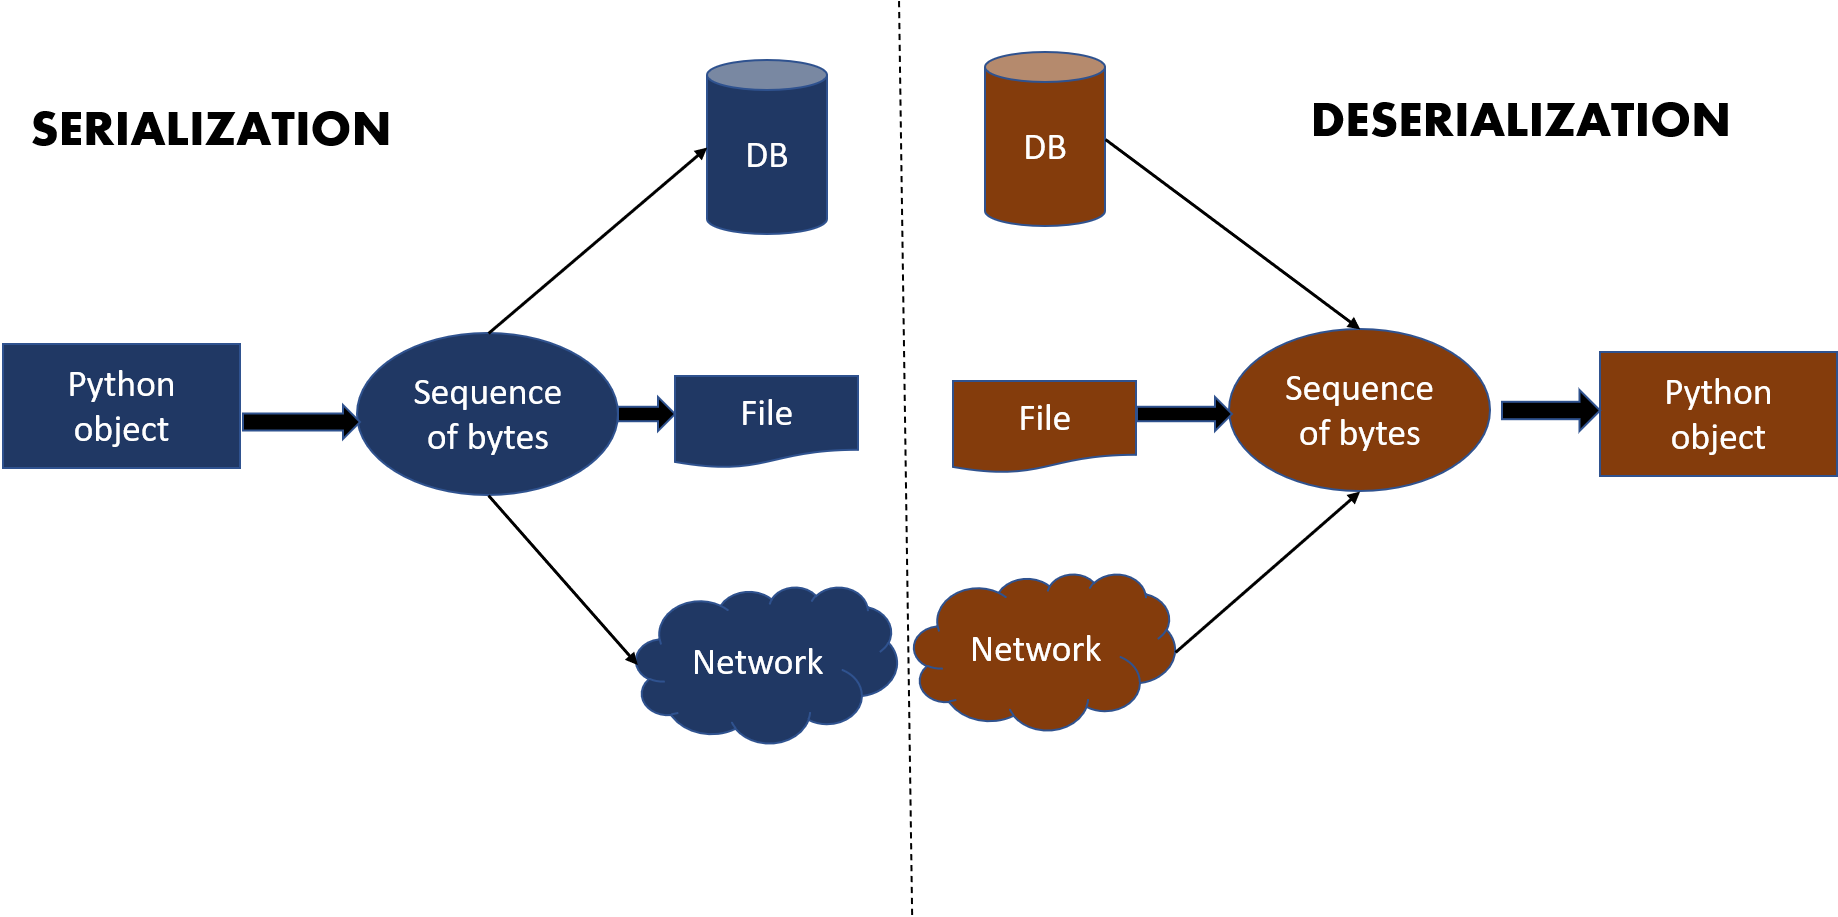
\includegraphics[width=0.8\textwidth]{images/serialization.png}
    \caption{(De)serialization}
    \label{fig:example-2}
\end{figure}

\newpage
\subsubsection{The \texttt{pickle} Module}
The \texttt{pickle} module provides functions for serializing and deserializing Python objects. It allows objects to be converted into a byte stream, which can then be saved to a file or transmitted over a network. The primary functions provided by the \texttt{pickle} module are:

\begin{itemize}
    \item \textbf{pickle.dump()}\\
    This function is used to serialize an object into a binary file. It takes two arguments: the object to be serialized and a file object (opened in binary write mode 'wb') to which the serialized data will be written. The function then writes the serialized data to the specified file, converting the object into a byte stream that can be saved to disk. Pickle is a module that provides serialization and deserialization functionalities.
    
    \item \textbf{pickle.load()}\\
    This function is used to deserialize an object from a binary file previously created using \texttt{pickle.dump()}. It takes a file object (opened in binary read mode 'rb') containing the serialized data as input and returns the deserialized object. The function reads the serialized data from the file and reconstructs the original object, effectively reversing the serialization process.
    
    \item \textbf{pickle.dumps()}\\
    This function is used to serialize an object into a byte stream representation, but it does \textbf{NOT write the data to a file}. Instead, it returns a byte string containing the serialized data.
    
    \item \textbf{pickle.loads()}\\
    This function is used to deserialize an object from a byte stream previously created using \texttt{pickle.dumps()}. It takes a byte string containing the serialized data as input and returns the deserialized object.
\end{itemize}



\begin{codebox}
\begin{minted}{python}
import pickle

class Fruit:
    def __init__(self, name: str, calories: float):
        self.name = name
        self.calories = calories
    
    def describe(self):
        print(self.name, self.calories, sep=': ')


# Create an instance of the Fruit class
banana: Fruit = Fruit('Banana', 100)

# Serialize the banana object and write it to the 'data.pickle' file
with open('data.pickle', 'wb') as file:
    pickle.dump(banana, file)
    
# Deserialize the object from the 'data.pickle' file
with open('data.pickle', 'rb') as file:
    fruit: Fruit = pickle.load(file)

fruit.describe() # Output: Banana: 100
\end{minted}
\end{codebox}


\newpage
The \texttt{pickle} module supports the serialization of various data types, including:

\begin{itemize}
    \item \textbf{Basic Data Types}\\
    Python's basic data types such as integers, floats, strings, and booleans can be easily serialized using the \texttt{pickle} module.
    
    \item \textbf{Lists, Tuples, and Dictionaries}\\
    Lists, tuples, and dictionaries, which are fundamental data structures, can also be serialized using \texttt{pickle}. This allows complex data structures to be stored and retrieved as a single object.
    
    \item \textbf{Custom Objects}\\
    Custom objects created by the user can also be serialized using \texttt{pickle}, provided that they are properly defined and their attributes are serializable. This allows entire object graphs to be stored and reconstructed later.
    
    \item \textbf{Functions and Classes}\\
    Functions and classes can be pickled as well, although there are limitations on what can be serialized. For instance, functions and classes defined at the top level of a module can typically be pickled, but dynamically created functions or classes may not be picklable.
\end{itemize}

\subsubsection{The \texttt{shelve} Module}
The \texttt{shelve} module provides a simple interface for managing persistent storage of Python objects. It allows you to store and retrieve objects from a file using key-value pairs, similar to a dictionary. It is particularly useful for applications that need to store data between program executions without requiring the complexity of a relational database.\\

\begin{codebox}
\begin{minted}{python}
import shelve

with shelve.open('TestDB') as db:
    db['one'] = 1
    db['two'] = 2
    db['three'] = 3

with shelve.open('TestDB') as db:
    print(type(db))
    print(dict(db))
    print(db['three'])
\end{minted}
\end{codebox}


\begin{minted}[
    bgcolor=white, % Background color
    frame=leftline, % Border style (only on left and right sides)
    framesep=2mm, % Padding around the frame
    rulecolor=black, % Border color
    linenos=false, % Disable line numbering
]{text}
<class 'shelve.DbfilenameShelf'>
{'one': 1, 'two': 2, 'three': 3}
3
\end{minted}

\textbf{Note}: The \texttt{shelve} module uses the \texttt{pickle} module internally for serializing and deserializing Python objects to and from the shelf file.

\newpage
\subsubsection{Storing Dictionaries with \texttt{shelve}}
This code defines a \texttt{Fruit} class with attributes for name and calories. It creates a dictionary of fruit objects and stores it persistently using the \texttt{shelve} module. 

\begin{codebox}
\begin{minted}{python}
import shelve

class Fruit:
    def __init__(self, name, calories):
        self.name = name
        self.calories = calories


data: dict = {
    'apple': Fruit('Apple', 10),
    'banana': Fruit('Banana', 100),
    'orange': Fruit('Orange', 50)
}

# Store fruits data
with shelve.open('FruitsDB') as db:
    db.update(data)
\end{minted}
\end{codebox}

\subsubsection{Retrieve Data from the shelf}
This code retrieves data from a persistent storage called a "shelf", specifically from a shelf file named \texttt{FruitsDB}.
\begin{codebox}
\begin{minted}{python}
import shelve

with shelve.open('FruitsDB') as db:
    # Retrieve the apple object
    apple: Fruit = db['apple']
        
    # Retrieve the banana object using the .get() method
    banana = db.get('banana')
    lemon = db.get('lemon')  # Returns None if the key does not exist
    
    # If key doesn't exist, it will add it with a default value of -1
    pomegranate = db.setdefault('pomegranate', -1)
    
    
# Prints the calories count of apple
print("Calories in an apple:", apple.calories)  # Output: 10
\end{minted}
\end{codebox}

%%%%%%%%%%%%%%%%%%%%%%%%%%%%%%%%%%%%%%%%%%%%%%%%%%%%%%%%%%%%%%%%%%%%%%%%%%
% 1.9
\newpage
\subsection{Exceptions}

\subsubsection{Errors}
Errors can be raised explicitly using the \texttt{raise} statement. This feature allows developers to generate exceptions when certain conditions are met, granting greater control over error handling within their code.

\begin{codebox}
\begin{minted}{python}
raise SomeException("Error message")
\end{minted}
\end{codebox}

\subsubsection{BaseException}
BaseException is the base class for all built-in exceptions. It serves as the superclass for all exceptions defined, including both system-defined exceptions (like ZeroDivisionError, TypeError, ValueError, etc.) and user-defined exceptions.

\begin{figure}[h!]
    \centering
    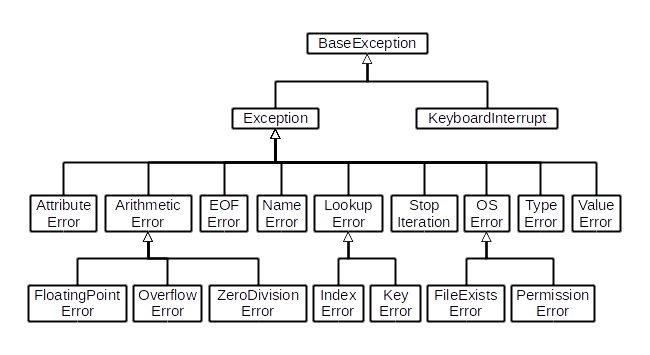
\includegraphics[width=0.95\textwidth]{images/exceptions.png}
    \caption{BaseException}
    \label{fig:example-3}
\end{figure}

\subsubsection{Exceptions as Objects}
In many programming languages, including Python, exceptions are represented as objects. An exception object encapsulates information about an exceptional event that has occurred during the execution of a program. This object typically contains details such as the type of exception, a message describing the error, and sometimes additional data relevant to the specific exception.

\newpage
\subsubsection{Exceptions}
Exceptions are used to handle errors and unexpected situations that may occur during the execution of a program. Using \texttt{try} and \texttt{except} blocks allows to handle errors, preventing the program from crashing and providing useful feedback to the user. It's a fundamental tool for writing robust and reliable code.
\begin{codebox}
\begin{minted}{python}
try:
    x = int(input("Please enter a number: "))
    result = 10 / x
    print("Result:", result)
    
except ZeroDivisionError:
    print("Error: Cannot divide by zero!")
    
except ValueError:
    print("Error: Please enter a valid number!")
\end{minted}
\end{codebox}

\begin{itemize}
    \item \textbf{\texttt{try:}} The \texttt{try} block contains the code that you want to execute. It is the part of the code where you anticipate an error might occur. If an exception occurs within this block, Python will stop executing the code in the \texttt{try} block and move to the \texttt{except} block.
    \item \textbf{\texttt{except:}} The \texttt{except} block is used to handle exceptions raised in the preceding \texttt{try} block. You can specify the type of exception you expect to occur. If the specified exception occurs in the \texttt{try} block, Python will execute the code in the \texttt{except} block.
\end{itemize}

\subsubsection{Named Attributes of Exception Objects}
Exception objects often have named attributes that provide information about the nature of the exception. These attributes can vary depending on the programming language and the specific exception type, but common attributes include:
\begin{itemize}
    \item \textbf{Type:} Indicates the type of exception that occurred. This could be a built-in exception type provided by the language or a custom exception type defined by the programmer.
    \item \textbf{Message:} A human-readable description of the error that occurred. This message often provides details about what went wrong and can be helpful for debugging.
    \item \textbf{Stack Trace:} A traceback or stack trace provides information about the sequence of function calls that led to the exceptional condition. It includes the file names, line numbers, and function names of the code where the exception occurred, helping developers pinpoint the source of the error.
    \item \textbf{Error Code:} Some exceptions may include an error code that provides additional context or categorization for the error.
    \item \textbf{Additional Data:} Depending on the exception type and the needs of the programmer, exception objects may contain additional data relevant to the exceptional condition. This could include input values, state information, or any other details that might be useful for handling the exception.
\end{itemize}

\subsubsection{Custom Exceptions}
Custom exceptions can be created to handle specific cases that are not covered by built-in exceptions.
\begin{codebox}
\begin{minted}{python}
# Custom exception class by inheriting from the built-in Exception class
class CustomException(Exception):
    def __init__(self, message="An error occurred"):
        self.message = message
        super().__init__(self.message)

# Example function that raises the custom exception
def example_function(number):
    if number < 0:
        # Raise the custom exception if the input is negative
        raise CustomException("Number cannot be negative")

try:
    # Call function with a negative number to trigger the custom exception
    example_function(-5)
except CustomException as e:
    # Handle the custom exception
    print("Custom Exception Caught:", e.message)
\end{minted}
\end{codebox}

\subsubsection{Chained Exceptions}
Chained exceptions, also known as nested exceptions or exception chaining, refer to the practice of capturing and preserving information about one exception while throwing another. This mechanism is particularly useful in scenarios where an error occurs within the context of handling another error.

Many modern programming languages and frameworks support chaining exceptions directly in their exception handling mechanisms. For example you can chain exceptions using the \texttt{raise} statement with the \texttt{from} keyword:

\begin{codebox}
\begin{minted}{python}
try:
    # Code that may raise Exception A
    raise Exception("Exception A occurred")
except Exception as e:
    try:
        # Code that may raise Exception B
        raise ValueError("Exception B occurred") from e
    except ValueError as ve:
        # Handle or re-raise Exception B
        print("Caught ValueError:", ve)
\end{minted}
\end{codebox}

In the above example, Exception B is raised with Exception A chained to it using the \texttt{from} keyword. This preserves the traceback information of Exception A while raising Exception B.

Chained exceptions are beneficial for understanding the flow of errors in a program and can greatly assist in debugging complex systems. However, it's essential to use them judiciously and avoid excessive nesting, which can make the code harder to follow.

\newpage
\subsubsection{The \texttt{\_\_cause\_\_} and \texttt{\_\_context\_\_} Attributes}
The \texttt{\_\_cause\_\_} and \texttt{\_\_context\_\_} are attributes of the exception object (\texttt{ve} in this case) that provide information about the relationships between exceptions.

\begin{itemize}
    \item \textbf{\texttt{\_\_cause\_\_}}: This attribute refers to the exception that caused the current exception to occur. It is used to indicate that the current exception was raised in direct response to another exception. In the given code, \texttt{ve.\_\_cause\_\_} prints the original exception (\texttt{Exception A}) that caused the \texttt{ValueError} exception (\texttt{Exception B}) to be raised.
    
    \item \textbf{\texttt{\_\_context\_\_}}: This attribute refers to the exception that was being handled when the current exception was raised. It provides context for the current exception. In the given code, \texttt{ve.\_\_context\_\_} would print \texttt{None} because there's no explicitly defined context for the \texttt{ValueError} exception. If there were an outer \texttt{except} block handling another exception, the exception object from that outer block would be accessible via \texttt{\_\_context\_\_}.
\end{itemize}


\begin{codebox}
\begin{minted}{python}
try:
    # Code that may raise Exception A
    raise Exception("Exception A occurred")
except Exception as e:
    try:
        # Code that may raise Exception B
        raise ValueError("Exception B occurred") from e
    except ValueError as ve:
        # Handle or re-raise Exception B
        print("Caught ValueError:", ve)
        print(ve.__cause__)
        print(ve.__context__)
\end{minted}
\end{codebox}


\begin{minted}[
    bgcolor=white, % Background color
    frame=leftline, % Border style (only on left and right sides)
    framesep=2mm, % Padding around the frame
    rulecolor=black, % Border color
    linenos=false, % Disable line numbering
]{text}
Caught ValueError: Exception B occurred
Exception A occurred
Exception A occurred
\end{minted}

\subsubsection{Implicitly and Explicitly Chained Exceptions}
Chained exceptions, both implicit and explicit, provide a way to maintain a history of exceptions that have occurred during program execution. This feature helps developers to debug and understand the flow of exceptions in their code more effectively.

\begin{itemize}
\item \textbf{Implicitly Chained Exceptions}\\ Implicitly chained exceptions occur when an exception is raised within the except block without explicitly specifying the original exception as the cause. In this case, Python automatically chains the new exception to the original one.
\item \textbf{Explicitly Chained Exceptions}\\
You can explicitly raise a new exception while capturing the original exception to provide more context. This is done using the \texttt{raise ... from ...} syntax. 
\end{itemize}

\newpage
\subsubsection{The \texttt{\_\_traceback\_\_} Attribute}
The \texttt{\_\_traceback\_\_} attribute of an exception object contains the traceback information associated with that exception. The traceback provides a detailed record of the execution path that led to the exception, including the sequence of function calls and the line numbers where the exception occurred.

\begin{codebox}
\begin{minted}{python}
import traceback

def function_with_error():
    # Some code that may raise an exception
    raise ValueError("An error occurred in function_with_error")

try:
    function_with_error()
except ValueError as e:
    # Accessing the __traceback__ attribute
    tb = e.__traceback__
    # Printing the traceback using the traceback module
    print(traceback.format_tb(tb))
\end{minted}
\end{codebox}

The traceback module provides functions to work with traceback objects.

\begin{itemize}
    \item \texttt{traceback.print\_tb(tb)}: Prints the traceback information to the standard output.
    \item \texttt{traceback.format\_tb(tb)}: Returns a formatted string containing traceback information.
    \item \texttt{traceback.extract\_tb(tb)}: Returns a list of tuples representing traceback information. Each tuple contains filename, line number, function name, and source line.
\end{itemize}

\subsubsection{Operating with different kinds of Exceptions}
The code efficiently handles potential errors by incorporating separate blocks for different types of exceptions, ensuring readability through clear separation and descriptive comments. Additionally, it adheres to Python's PEP 8 style guide for code layout, enhancing overall clarity and maintainability.
\begin{codebox}
\begin{minted}{python}
try:
    # Your code that may raise exceptions
    x = int(input("Enter a number: "))
    y = 10 / x
    print("Result:", y)

except ValueError:
    # Handle ValueError (invalid input)
    print("Please enter a valid integer.")

except ZeroDivisionError:
    # Handle ZeroDivisionError (division by zero)
    print("Cannot divide by zero.")

except Exception as e:
    # Catch any other unexpected exceptions
    print("An error occurred:", e)
\end{minted}
\end{codebox}






